% ============================================================================
% Chapter 5 · Discussion
% ============================================================================

\section{Discussion}\label{sec:discussion}

This chapter answers the three research questions against the evidence of
Chapter 4, sets those answers against the literature and gives the limits of the work and what follows
from them.

\subsection{Answers to the research questions}\label{sec:one_figure}

\textbf{The first question asks how capture value in the enclosed Baltic
compares with the open North Sea today, and how it changes under the committed
buildout to 2030 and 2040.} The two basins are level today: offshore farms in
the under-built Baltic zones capture 0.883 of the average wholesale price
against 0.879 in the North Sea, which is to say that a farm in either basin
received close to 88 per cent of the price a plant generating continuously
would have received over the same period. The fall is modest to 2030 and steep
after it. By 2040, under National Trends, the pathway of the official plan
that tracks existing national policies, the Baltic falls to 0.47 while the
North Sea holds 0.57, so a basin that begins level has lost close to half of
the value it captures today. That outcome depends on the network built
alongside the farms, since with transmission free to expand the Baltic
recovers to 0.66 against the North Sea's 0.64. How much grid is built therefore decides how far the Baltic
falls behind, although even under the most favourable grid tested it still
captures about 0.2 points less than it does today.
Figure~\ref{fig:group_arc} shows the measured record and the projection in one
view.

\begin{figure}[!htb]
    \centering
    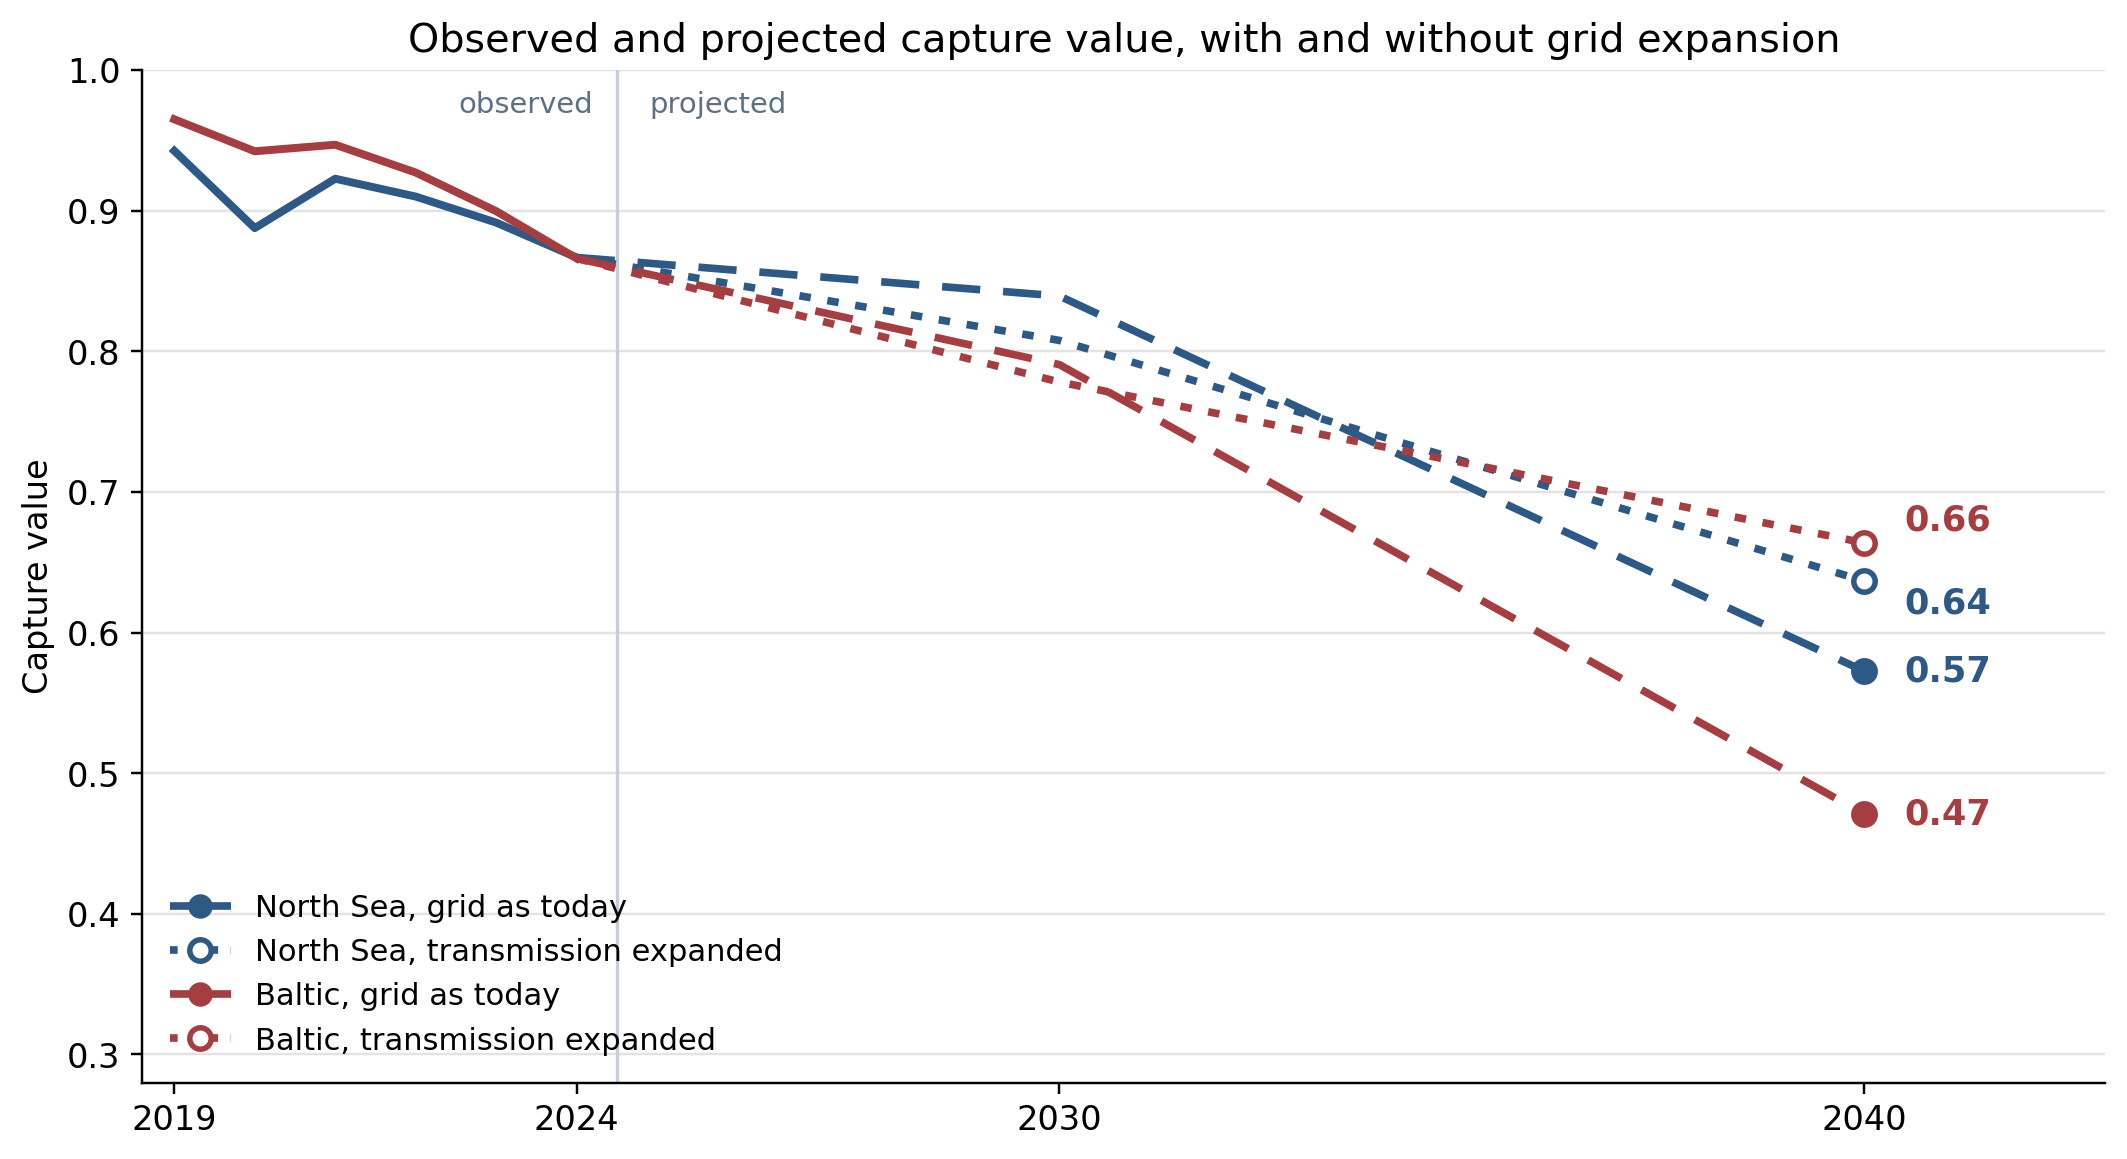
\includegraphics[width=0.95\textwidth]{image-1787753091449.png}
    \caption{Capture value for the North Sea and the Baltic, measured to 2024
    and projected to 2040 under National Trends with the scheduled buildout,
    on today's grid. Solid lines are observed values and dashed lines the
    projection. The Baltic line covers the zones that build out, Poland,
    Estonia, Latvia and Lithuania. The full scenario set and the corrected
    values are in Section~\ref{sec:corrected_projection} and
    Appendix~\ref{app:robustness}.}
    \label{fig:group_arc}
\end{figure}

\textbf{The second question asks which mechanisms set the rate at which capture
value is eroded, whether they differ between an enclosed and an open basin, and
how much of that erosion system design can remove.} Between individual farms the
largest single cause is crowding, meaning how closely a farm's output coincides
with that of the rest of the system, since a farm generating when everything
else generates is selling into hours in which the price has already been driven
down. The same mechanisms operate in both basins and are simply stronger in the
Baltic, where the penalty for generating alongside everything else is twice as
large as in the North Sea.

A substantial part of the resulting loss can be removed by building differently.
Of the 0.42 the Baltic loses under National Trends, 0.19 is congestion that an
expanded grid removes while 0.23 comes from the buildout itself, so nearly half
of the loss follows from the network around the basin. Allowing demand to shift
in time recovers a comparable amount to expanding the grid, 0.28 against 0.19,
which means the two levers available to a system planner are of similar size
(Table~\ref{tab:drivers}).

\begin{table}[!htb]
\centering\small
\caption{The Baltic fall attributed, in the 2040 National Trends scenario
unless stated otherwise. Each component is measured in the section given. The
last two rows are the two design levers, and they add value.}
\label{tab:drivers}
\begin{tabular}{l c l}
\toprule
\textbf{Component} & \textbf{Capture value} & \textbf{Section} \\
\midrule
Total fall, today to 2040 on today's grid & $-0.42$ &
\S\ref{sec:corrected_projection} \\
\quad the buildout itself, which no grid removes & $-0.23$ &
\S\ref{sec:decomposition} \\
\quad congestion, which an expanded grid removes & $-0.19$ &
\S\ref{sec:decomposition} \\
Scarcity pricing inside the stressed scenarios & up to $-0.15$ &
\S\ref{sec:scarcity_results} \\
Winter concentration (winter 0.50, summer 0.83) & seasonal &
\S\ref{sec:seasonality} \\
Recovered by expanding transmission & $+0.19$ & \S\ref{sec:grid_results} \\
Recovered by fully flexible demand & $+0.28$ & \S\ref{sec:sector_results} \\
\bottomrule
\end{tabular}
\end{table}

\textbf{The third question asks whether a model trained on historical
observation can project these futures, whether a system model is required, and
how the two should be combined and validated against each other.} A model
trained on observation cannot project them, and the reason lies in what each
kind of model contains.

The regression model learns a relationship between seven market conditions and
capture value from prices that have already occurred, which is why it reproduces
the recent record more closely than the system model does. The model has
inherited that accuracy from the record, and it holds only while conditions
resemble the ones the model was fitted on. Once the system changes
fundamentally, the association the model learned no longer describes the system
it is being asked about.

The system model contains no fitted relationship at all. It is assembled from
the plants and what it costs to run them, the network and what it can carry, and
demand in every hour, and it re-derives the price in each hour by finding the
cheapest way to meet that demand. Because the mechanism is built in, changing
the fleet changes the answer for the right reason, and the model responds to a
scenario that has never occurred. The price of building the mechanism is that it
must be simplified before it can be solved.

The measurements support this account of the two models, since over the
observed record the two are equally accurate, each missing observed capture value by about 0.04 on average across
144 combinations of zone and month that neither had been fitted on
(Table~\ref{tab:skill}). Beyond that record 90 per cent of their disagreement
at 2040 comes from the regression model no longer responding to the scenario,
while the two continue to agree on how prices are formed. To locate that
boundary, the regression model was refitted on data ending in 2021 and asked
for 2023 and 2024. The two models projected those years equally well, since
most of the targets still lay inside the conditions the regression model had
seen, so the limit is the edge of the observed record rather than the number
of years ahead.

Their construction assigns their roles (Table~\ref{tab:models}). The regression
model, fitted to 2,706 monthly observations from 31 farms, measures the present
and forecasts over horizons short enough that market conditions remain
recognisable. The system model, solved hourly across thirty nodes under official
capacity trajectories, is the only instrument that can price the 2040 fleet, and
it carries the projection with its measured overstatement subtracted.
\subsection{Findings in relation to the literature}\label{sec:disc_literature}

The flexibility offered by hydro was expected to protect the Baltic from a sharp
decline in capture value, and it does not. Hirth finds that systems with a large
hydro fleet hold wind value better than systems built on gas and coal, by about
eighteen percentage points of capture value once wind reaches 30\,\% of supply,
because reservoirs absorb the surplus produced on windy days \cite{Hirth2013}.
The Baltic has that hydro, so on Hirth's reasoning its zones should capture more
of the average price than the North Sea's, whereas the measured record puts the
two level at 0.883 against 0.879 with almost none of the Baltic's offshore
pipeline yet built (Table~\ref{tab:archetype_measured}). The
expectation was built into the design of this thesis, since the archetype table
of Chapter 2 marked the hydro-buffered markets as favourable before the
measurement was made. The explanation is one of scale, since the storage available around the Baltic is small relative to the
surplus a full buildout would produce, and once that storage is full the
remaining power has nowhere to go, because the basin has little capacity to
export it. Hirth's effect operates within a market, and the difficulty in the
Baltic is moving power out of one.

The projection reported falls further than any published for a European
offshore basin. The Baltic's central 0.47 in 2040 sits below the worst North Sea
case Jacquet reports \cite{Jacquet2024}, and it does so at the resolution at
which prices are set, where earlier work reports national averages. The same work
identifies winter as the season in which cannibalisation concentrates, and the
results sharpen that finding, because the two seas are windy at the same
time in winter, so export capacity is least useful in the months when output is
highest, and by 2040 almost the entire annual loss falls in that season, at 0.50
in winter against 0.83 in summer.

Efthymiadou's finding for the United Kingdom, that it is how much
interconnection is actually used, and not the presence of the capacity alone,
that steadies prices \cite{Efthymiadou2025}, is extended here, since relieving the transmission constraint
lifts the most stressed 2040 scenarios by about 0.2 in capture value while
allowing demand to move in time is worth a comparable amount. Those two changes
to the physical system are the largest levers identified anywhere in this work.
Stiewe et al.\ represent the influence of neighbouring markets as a single fixed
coefficient for each zone \cite{Stiewe2025}, which holds that influence constant
over time, whereas in this case the same penalty grows as more capacity is built and can
be separated into the part congestion causes and the part the buildout causes.

Every published benchmark sits above the values projected, whether Hirth's
range of 0.5 to 0.8 at a 30\,\% share \cite{Hirth2013}, Germany's measured 0.76
at 35\,\% \cite{Stiewe2025, Ember2025}, or the roughly 0.6 of Jacquet's worst
North Sea case \cite{Jacquet2024}. Each of those was measured in a more open
market and at a lower level of wind than the Baltic reaches in these scenarios,
so the difference between them reflects where each sits on the same curve. The
panel literature reinforces that reading, having established that the decline
steepens as penetration rises \cite{LopezProl2024, Cevik2022}, which extends the
published trajectories into the range projected.

The two models behaved as the literature predicts in one respect and not in the
other. A model fitted to data is conventionally expected to understate the
spread of the observations, while a model built from physical and cost
relationships is expected to carry a consistent offset \cite{Theil1966}. The
system model behaves as expected, reading consistently too high by 0.041 on
average, but the regression model does not, since it reproduces the spread of
the observations accurately and its error lies almost entirely in which months
it places high and which low. What it has learned, in other words, is how much
cannibalisation there is without learning when it occurs, which is a more
forgiving failure when the task is to measure today's level than when the task
is to rank one month against another.

\subsection{Limitations and future directions}\label{sec:conc_limitations}

The complete register of assumptions is given in Appendix~\ref{app:assumptions}.
The limitations capable of altering a reported value are set out below, each
with the work that would resolve it.

The bias correction is fitted on a single high-penetration zone. DK2 is the only
validation point at an offshore share comparable to the projected Baltic, and
removing it leaves a correction that no longer increases with buildout, so the
correction is reported as a refinement and the values quoted throughout
come from the uncorrected system model (Appendix~\ref{app:robustness}).
Resolving this requires further validation points at high penetration, which
will become available as the Baltic fleet is commissioned.

The system model solves a linear dispatch and does not represent
generating units that must remain online or that bid below their marginal cost.
This is the source of the overstatement in DK2, and replacing the assumed
interconnector ratings with the capacities offered to the market corrects DK1
without correcting DK2. Representing unit commitment and must-run heat
production explicitly would address it directly, at a substantial increase in
computational cost.

The accounting of who bears the loss covers generated energy only and does not
include curtailed volume, which amounts to a third of North Sea wind output on
the 2040 network held at today's capacity. Including curtailed energy, and
solving at intermediate levels of network expansion so that the planned network
is priced alongside the present and the fully expanded cases, would complete
that accounting.

Great Britain and Norway do not pass validation at the spatial resolution used and are excluded from every reported aggregate, although the three British
farms remain in the regression model's training data up to 2020, when British
prices left the ENTSO-E platform. Great Britain is a suitable subject for a
separate application of the same design, since its market record is public and
nothing after 2020 has been used.

Only DK2 and one Swedish farm have operating offshore capacity in the enclosed
Baltic, so the remaining zones are represented by the validated virtual wind
farm, since local measurement does not exist there. The regression model nevertheless
predicts six of the seven enclosed zones to within 0.07 of the observed value
when those zones are withheld from fitting, and metered output from the farms
now under construction would allow this to be tested directly.

The projection holds the correlation between wind patterns and the utilisation
of interconnection fixed at present values, and the fast approximation used for
the wider scenario sweep becomes optimistic at the highest levels of buildout.
For both reasons the values reported come from the direct zone-by-zone solves,
with the present network and the fully expanded network bounding the result.

Two extensions follow from this work. The first is geographic. The design uses
open data, an open resource model and an open system model throughout, so it can
be applied wherever hourly prices and a network representation exist, and
extending it beyond the two basins studied in this work would allow offshore potential
to be assessed on the value of the electricity produced rather than on the wind
resource alone, across a considerably wider set of markets. The second concerns
sector coupling. The sector-coupled solve reported is a single sensitivity,
and it shows that flexible demand recovers as much capture value as network
expansion does, which makes the assumption about future flexibility one of the
largest open questions in the result. Running the complete scenario set in
PyPSA-Eur-Sec, rather than as a bracket applied to one case, would establish how
much of the projected erosion survives once heat, transport and hydrogen demand
are optimised alongside electricity.